%% \section{The blinkered policy}

%% This is the key section.  Write it, and then see what prereqs are required.

The myopic policy is an extreme approximation, often stopping significantly early.
For a natural class of metalevel probability models we can define a better approximation:

\begin{dfn}\label{dfn:independent-actions}
	A metalevel probability model $\mathcal{M}=(U_1,\dots,U_k,\Evidence)$ 
	has \term{independent actions} if the computational variables can be partitioned 
	$\Evidence = \Evidence_1\cup\dots\cup\Evidence_k$ such that such that
	the sets $\{U_i\}\cup\Evidence_i$ are independent of each other for different $i$.	
\end{dfn}

\begin{dfn}\label{dfn:blinkered}
	Given a metalevel decision problem $M=(S,s_0,A_s,T,R)$ with independent actions,
	the \term{blinkered policy} $\pi^b$ is defined by $\pi^b(s) = \argmax_{a\in A_s} Q^b(s,a)$ where
	$Q^b(s,\bot) = \bot$ and for $E_i\in\Evidence_i$
	\begin{equation}\label{eq:blinkered}
		Q^b(s,E_i) = \sup_{\pi\in\Pi^b_i} Q^\pi(s,E_i)
	\end{equation}
	where $\Pi^b_i$ is the set of policies $\pi$ where $\pi(s)\in\Evidence_i$ for all $s\in S$.
\end{dfn}

This is a better approximation than the myopic policy as it takes into account more possible future strategies.
Indeed, $Q^m(s,a) \le Q^b(s,a) \le Q^*(s,a)$.  Intuitively, whereas the myopic policy can only see one 
computation ahead, the blinkered policy can see arbitrary far ahead but with blinkers on so can only see
the computations involving a single action at a time.



\begin{dfn}\label{dfn:one-action}
	Given a metalevel decision problem $M=(S,s_0,A_s,T,R)$ with independent actions,
	a \term{one-action metalevel decision problem} for $i=1,\dots,k$ is the metalevel decision
	problem $M^1_{i,m} = (S_i,s_0,A_{s0},T_i,R_i)$ defined by the metalevel probability
	model $(U_0,U_i,\Evidence_i)$ with $U_0=m$.
\end{dfn}

Note that given that state $s$ of a metalevel decision problem, we can form a state
$s_i$ by taking only the results of computations in $\Evidence_i$ (see \dfnref{dfn:metalevel-mdp}).
By action independence, $\mu_i(s)$ is a function only of $s_i$.

\begin{thm}\label{thm:blinkered}
Given a metalevel decision problem $M=(S,s_0,A_s,T,R)$ with independent actions,
let $M^1_{i,\mu}$ be the $i$th one-action metalevel decision problem for $i=1,\dots,k$.
Then for any $s\in S$, whenever $E_i\in A_s\cap\Evidence_i$ we have:
\[
	Q^b_M(s,E_i) = Q^*_{M^1_{i,m_i}}(s_i, E_i)
\]
where $m_i = \max_{j\neq i} \mu_i(s)$.
\end{thm}

\begin{comment}
	\begin{proof}
	Fix a state $s$, a $E_i\in A_s$ and take any $\pi\in\Pi^b_i$.  Note that such policies
	are equivalent to polices $\pi'$ on $M^1_{1,m}$, and all such policies are represented.
	Consider $Q^\pi(s,E_i)$.  As $\pi(s)\in\Evidence_i$ for all $s\in S$, by action independence $\mu_j(S_n) = \mu_j(s)$.
	By this and \thmref{thm:value-of-computation}, then,
	\[
		Q^\pi(s,E_i) = \IE^\pi_M[ -c\,N + \max(\mu_i(S_N), m_i) \given S_0=s, A_0=E_i].
	\]
	Noting that $\mu_i(S_N)$ is a function only of $(S_N)_i$, and that since 
	But then this is exactly $Q^{\pi'}_{M^1_{i,m_i}}(s_i, E_i)$.  Taking the supremum
	over $\pi$ gives the result.
	\end{proof}	
\end{comment}

\thmref{thm:blinkered} shows that to compute the blinkered policy we need
only compute the optimal policies for all $i$th one-action metalevel decision problems.

For the Bernoulli problem with $k$ actions, the one-action metalevel decision problems
are all one-action Bernoulli problems (\exampleref{example:bernoulli}).  By \thmref{thm:one-action-bound}
these policies perform at most $1/4c - 3$ computations.
As a result, the blinkered policy can be numerically computed in time $O(D/c^2)$ 
independent of $k$ by backwards induction, where $D$ is the number of points $m\in[0,1]$
we compute $Q^*_{M^1_{i,m}}(s)$ for\footnote{in our experiments below, $D=129$ points are equally spaced,
using linear interpolation between points}.  This will be worth the cost in 
the same situations as mentioned at the of \secref{sec:optimal}.

\figref{fig:blinkered} compared the expected regret of the blinked policy on the 
Bernoulli sampling problem with $k=25$ and varying cost of samples to several 
alternatives, where the regret include the cost of sampling:
\[
	R = (\max_i U_i) - U_j + c\,n
\]
if the policy performs $n$ computations and selects action $j$.
Myopic is the myopic policy for Bernoulli sampling. ESPb is the 
policy recently proposed by \citet{Chick+Frazier:2011}, which approximates the 
blinkered policy for sampling normal distributions by moving to continuous time
and numerically solving a diffusion equation.  UCB1-B uses UCB$(1/\sqrt2)$ \cite{Auer+et+al:2002} to
choose which actions to sample and the blinkered policy to stop.  UCB1-b uses
UCB$(1/\sqrt2)$ to sample, is given the average number of samples blinkered
uses for the given cost.

The blinkered policy significantly outperforms all others.  The myopic policy
plateaus as it quickly reaches a position where no single computation can
change the final decision between actions.  ESPb performs quite well given
that is making a normal approximation to the Beta posterior.  
UCB1-B and UCB1-b's curve shows that even given a good stopping rule, UCB1's
choice of actions to sample can be significantly improved on.


\begin{figure}[htb]
\centering
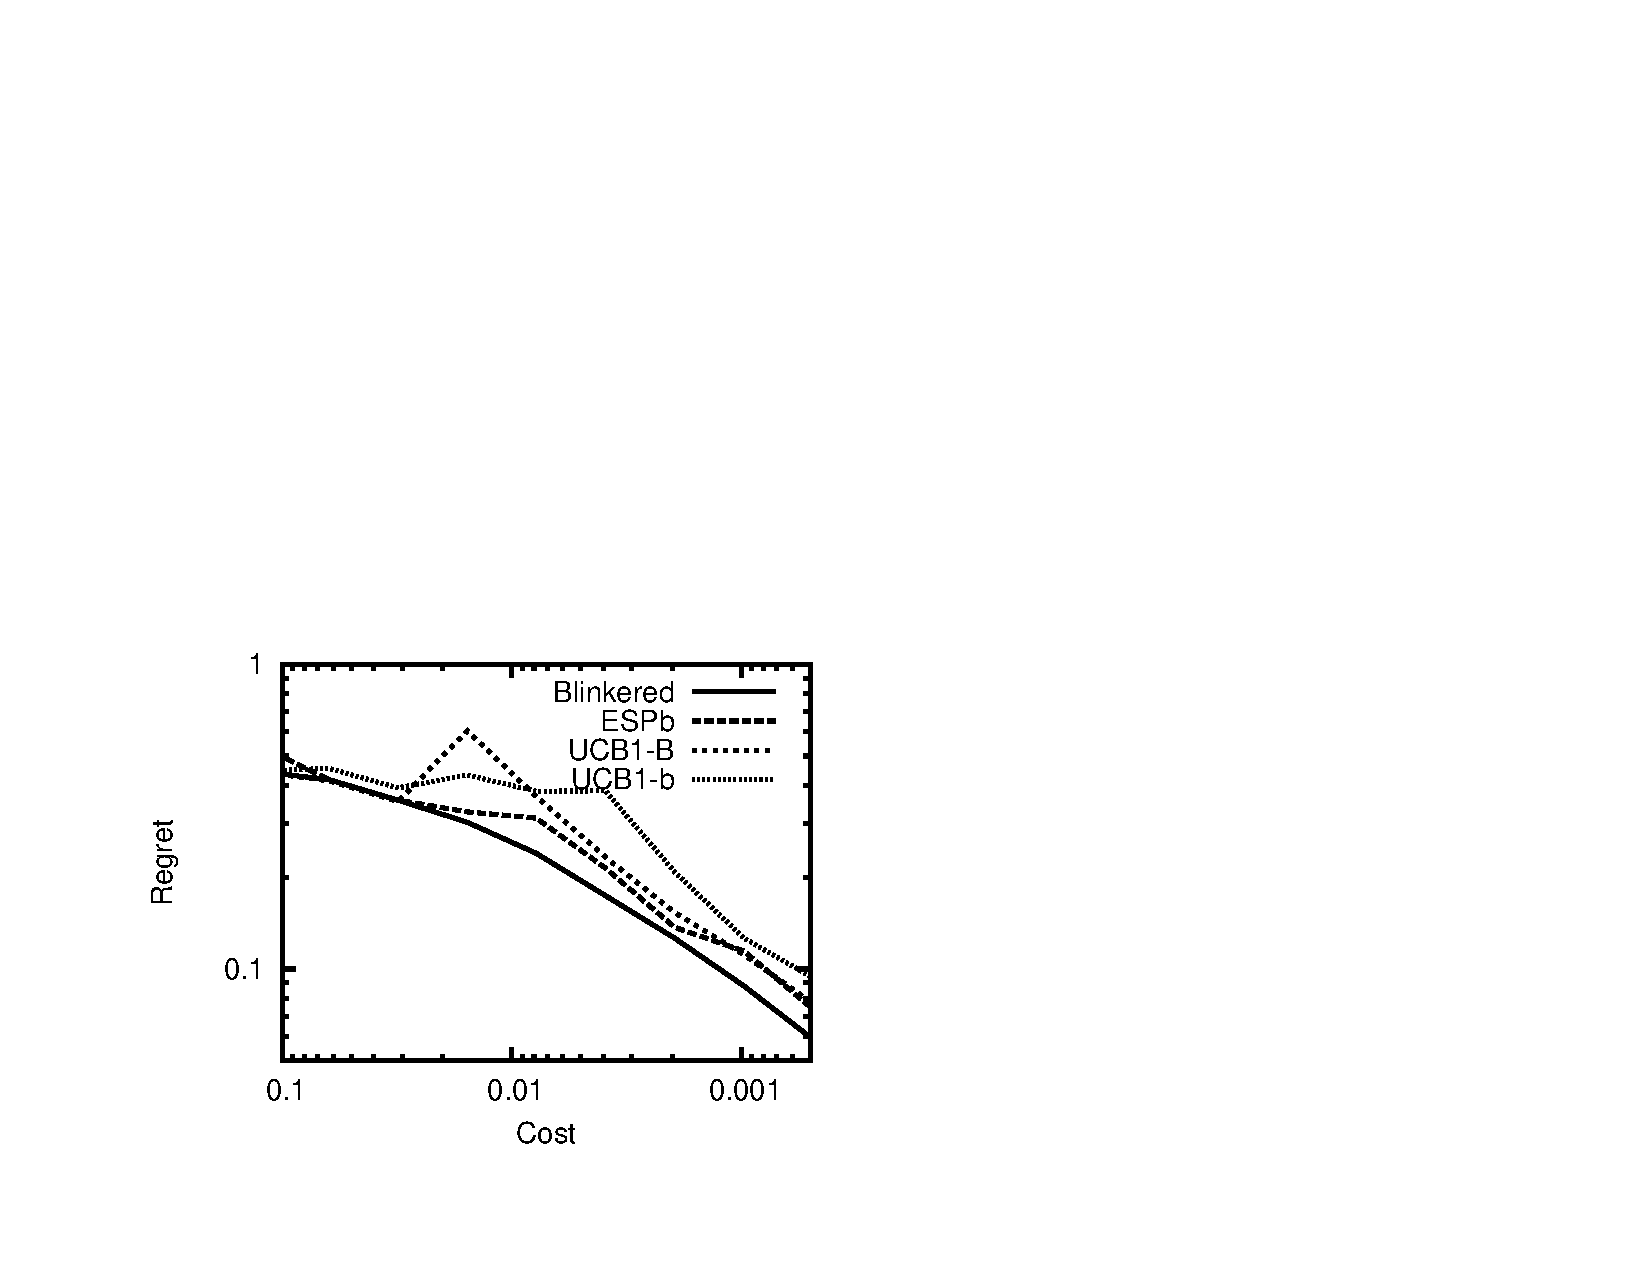
\includegraphics[scale=0.7, trim=90 70 400 300]{blinkered-regret.pdf}
\caption{Average regret of various policies as a function of the cost in 
a 25-action Bernoulli sampling problem.  Averaged over 1000 trials.}
\label{fig:blinkered}
\end{figure}

\begin{comment}
set xlabel "Cost"
set ylabel "Regret"

set terminal postscript enhanced linewidth 2
set output "blinkered-regret.ps"
set size 0.5, 0.5

set logscale xy

set key left bottom
plot [0.1:0.0005] [0.05:1] "blinkered-regret.dat" title "Blinkered" with lines lw 2, "myopic-regret.dat" title "Myopic" with lines lw 2, "espb-regret.dat" title "ESPb" with lines lw 2, "ucb-blinkered-regret.dat" title "UCB1-B" with lines lw 2, "ucb-blinkered-table-regret.dat" with lines lw 2 title "UCB1-b"
\end{comment}
